\section{\BRAG: Bodhi-Regularized Alignment Gradient}
\label{sec:algorithm}

\subsection{The algorithm}
Figure~\ref{fig:architecture} shows the data flow; Algorithm~\ref{alg:brag} gives one training run.
\BRAG{} is proximal policy optimization \cite{schulman2017ppo} of \eqref{eq:bodhi}.
The three critics $d_K$, $d_A$ and $h$ are computed from a model of the world---in the tabular case exactly, from reachability, from \POWER{} under sampled reward functions, and from the suffering function---and are \emph{frozen}: they are never updated on the agent's own trajectories (\S\ref{sec:lojong}).
Each iteration collects a batch of trajectories under the current (shield-masked) policy, shapes the rewards with the level penalty, estimates advantages of the shaped reward and of the suffering with generalized advantage estimation \cite{schulman2016gae}, combines them with a multiplier $\nu_k$, and takes a clipped surrogate step.
The multiplier is either a dual variable updated by projected ascent on the constraint violation (PPO-Lagrangian \cite{ray2019safety}),
\begin{equation}
\nu_{k+1}=\big[\nu_k+\eta_\nu\,(C(\pi_k)-\epsilon)\big]_+ ,
\label{eq:dual}
\end{equation}
or the gradient weight of a logarithmic barrier (IPO \cite{liu2020ipo}),
\begin{equation}
\nu_k=\frac{1}{t_k\,(\epsilon-C(\pi_k))},\qquad C(\pi_k)<\epsilon ,
\label{eq:barrier}
\end{equation}
with $t_k$ increasing over training.
The barrier requires every iterate to be feasible; we keep it so by a backtracking safeguard (if a proposed step would leave the feasible set the step is shortened, and if that fails a pure cost-descent step is taken) and by starting from the \emph{preliminaries} phase below.
In the tabular experiments the constraint cost $C(\pi_k)$ of each iterate is computed exactly from the model, as a model-based estimator would; estimating it from the batch is a standard component of both parent methods and not the object of study here.

\begin{figure}[t]
\centering
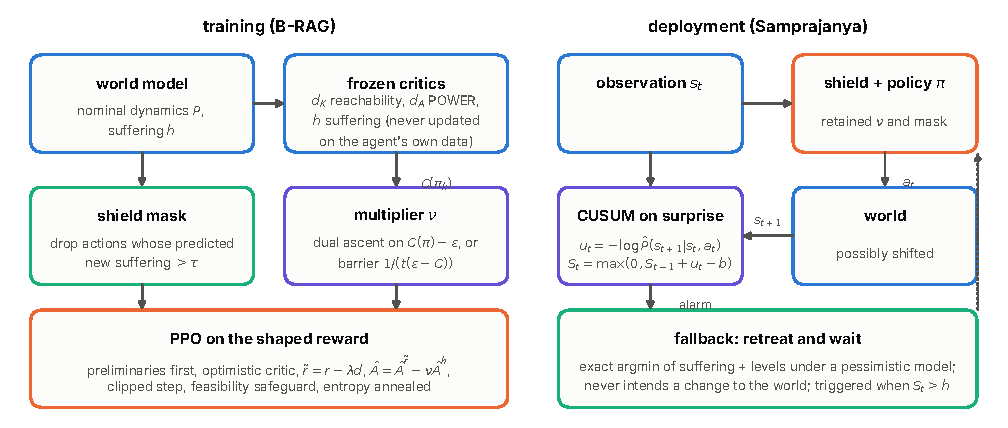
\includegraphics[width=\textwidth]{figs/fig_architecture.pdf}
\caption{Data flow. Training: a nominal world model yields three frozen critics; the shield masks actions whose predicted new suffering exceeds $\tau$; the multiplier is a dual variable or the barrier's gradient weight, computed from the exact constraint cost of the current policy; PPO optimizes the shaped reward after a preliminaries phase. Deployment: the policy keeps its mask and multiplier; a CUSUM on model surprise triggers a retreat-and-wait fallback.}
\label{fig:architecture}
\end{figure}

\begin{algorithm}[t]
\caption{\BRAG{} (one training run)}
\label{alg:brag}
\begin{algorithmic}[1]
\Require task MDP; frozen critics $d_K,d_A,h$; weights $\lambda,\alpha,\beta$; budget $\epsilon$; shield threshold $\tau$; multiplier mode (dual or barrier)
\State mask every action whose model-predicted one-step increase in suffering exceeds $\tau$ \Comment{pre-action shield}
\State initialize $\pi_\theta$ (uniform or inaction); task critic $V\gets v_0$ above any attainable return (optimistic); $\nu\gets0$
\State \textbf{preliminaries:} with a high entropy bonus, minimize the penalty $\E[\sum_t\gamma^t\lambda d(s_{t+1})]$ and the cost until the exact penalty level is below $\delta$ and $C(\pi)<0.8\,\epsilon$ \Comment{learn harmlessness first}
\For{$k=0,1,\dots,K-1$}
  \State collect trajectories under $\pi_\theta$; shaped reward $\tilde r_t=r_t-\lambda\,(\alpha d_K+\beta d_A)(s_{t+1})$
  \State GAE advantages $\hat A^{\tilde r}$ and $\hat A^{h}$ with learned values $V,V^h$
  \State $\nu\gets$ \eqref{eq:dual} (dual) or \eqref{eq:barrier} (barrier), using $C(\pi_\theta)$
  \State $\hat A\gets\hat A^{\tilde r}-\nu\,\hat A^{h}$, normalized
  \State $\theta\gets$ clipped-surrogate ascent on $\hat A$ with entropy bonus $\kappa_k$ (annealed) \Comment{proximal step}
  \If{barrier \textbf{and} $C(\pi_\theta)\ge\epsilon$} shorten the step; if still infeasible take a cost-descent step \EndIf
\EndFor
\State \Return $\pi_\theta$ together with $\nu$ and the shield \Comment{commitments are retained}
\end{algorithmic}
\end{algorithm}

Three features distinguish Algorithm~\ref{alg:brag} from a generic constrained-PPO recipe, and all come from the protocol of \S\ref{sec:lojong}.
The \emph{preliminaries} phase exists because the barrier needs a feasible start and because a disposition is installed before the task is pursued, not after: an agent that learns the task first and is regularized later has, by then, a near-deterministic policy and no data about the alternatives it is now asked to prefer (\S\ref{sec:lojongexp}).
The \emph{optimistic} task critic exists because persistent penalties encountered during random exploration otherwise teach an agent to stop moving before it has found anything worth moving for (\S\ref{sec:lojongexp}).
The \emph{retained} multiplier and shield exist because a commitment that is discarded at deployment is not a commitment.

\subsection{Why a barrier}
Dual ascent and the barrier are two ways of producing a multiplier.
The first two propositions say how they differ.

\begin{proposition}[The barrier is an adaptive multiplier]
\label{prop:barrier}
On the strictly feasible set $\{\theta: C(\theta)<\epsilon\}$ let $B_t(\theta)=J_\lambda(\theta)+\tfrac1t\log(\epsilon-C(\theta))$.
Then $\nabla_\theta B_t(\theta)=\nabla_\theta J_\lambda(\theta)-\nu(\theta)\nabla_\theta C(\theta)$ with $\nu(\theta)=1/(t(\epsilon-C(\theta)))$, which increases without bound as $C(\theta)\uparrow\epsilon$.
\end{proposition}

So a step of \BRAG{} in barrier mode is a Lagrangian step whose multiplier is a function of the current iterate rather than a state carried across iterates; it needs no step size, it reacts instantly, and it cannot be ``behind'' when the policy moves.
Its cost is that it is undefined outside the feasible set---hence the safeguard and the preliminaries.

\begin{proposition}[Optimality gap of the barrier]
\label{prop:gap}
Let $J^\star_c$ be the value of \eqref{eq:bodhi}, and suppose a strictly feasible policy exists.
In occupancy-measure space the problem is a linear program; let $\rho_t$ maximize $\langle\rho,\tilde r\rangle+\tfrac1t\log(\epsilon-\langle\rho,h\rangle)$ over feasible occupancy measures.
Then $\rho_t$ is feasible and $J^\star_c-\langle\rho_t,\tilde r\rangle\le 1/t$.
\end{proposition}

This is the standard interior-point bound \cite[\S11.2]{boyd2004convex} for one inequality constraint; the proof is in Appendix~\ref{app:proofs}.
It says what the barrier buys: a path of \emph{feasible} solutions whose suboptimality is controlled by a single number, so that increasing $t_k$ during training trades a little return for a lot of safety during training, with nothing to tune about how fast a multiplier should move.
The proposition concerns the exact barrier maximizer in occupancy space; the policy-gradient iterates approximate it, which is what \S\ref{sec:multiplier} measures.

\subsection{The abstention threshold}
\label{sec:threshold}
The soft terms are levels.
The following proposition gives the exact sense in which a level penalty deters an irreversible act, and by how much a persistent penalty beats a one-off one.

\begin{assumption}
\label{ass:acts}
$d\ge0$ vanishes on the clean set $\clean$.
A transition $(s,a)$ from $s\in\clean$ that can leave $\clean$ is an \emph{act}, and every act is an irreversible departure: every state reachable after it lies outside $\clean$ and has $d\ge\Omega>0$.
Some policy that never leaves $\clean$ exists from every clean state (e.g.\ inaction).
\end{assumption}

\begin{proposition}[Abstention threshold]
\label{prop:threshold}
Under Assumption~\ref{ass:acts}, let $V^\star_\varnothing(s)$ be the optimal task value among policies that never leave $\clean$ from $s$, and let the \emph{option premium} of the acts be
\begin{equation}
\tilde G=\max_{s\in\clean,\ (s,a)\text{ an act}}\ \big[Q^\star(s,a)-V^\star_\varnothing(s)\big].
\end{equation}
If
\begin{equation}
\lambda>\lambda^\star:=\frac{(1-\gamma)\,\tilde G}{\Omega},
\label{eq:threshold}
\end{equation}
then no optimal policy of the unconstrained regularized problem $\max_\pi J_\lambda(\pi)$ commits an act in any clean state; started in $\clean$, it stays in $\clean$.
\end{proposition}

\begin{corollary}[Level versus one-off]
\label{cor:oneoff}
If the penalty is instead charged once, as $\lambda\max(0,d(s_{t+1})-d(s_t))$, the same conclusion requires $\lambda>\tilde G/\Omega=\lambda^\star/(1-\gamma)$.
\end{corollary}

The proof (Appendix~\ref{app:proofs}) is two lines: from the act onward the agent pays at least $\lambda\Omega$ at every step, which is worth $\lambda\Omega/(1-\gamma)$ in discounted terms, while the most the act can have gained it is $\tilde G$; the one-off variant pays $\lambda\Omega$ once.
Three things about \eqref{eq:threshold} are worth stating.
It is \emph{computable}: $\tilde G$ and $\Omega$ are properties of the task and the critics, not of training, so the weight needed to deter a given act can be read off before any training happens (\S\ref{sec:sweep} checks the number).
It is \emph{sufficient, and tight when the level is uniform}: when every post-act state has level exactly $\Omega$ and the premium is realized at the threshold state, the bound is attained.
And it says what persistence buys: with $\gamma=0.95$ a level penalty deters at a weight twenty times smaller than a one-off penalty, because the one-off penalty is a single tax on a change whereas the level is a rent on the world the agent has made.
The assumption of irreversibility is used; for a reversible departure (the switch, which can be toggled back) the proposition does not apply as stated, and \S\ref{sec:sweep} shows what happens instead.

\subsection{Why the power term must be one-sided}
\label{sec:onesided}
Section~\ref{sec:setting} argued informally that a symmetric power penalty is a self-preservation incentive.
The argument is exact.

\begin{proposition}[Symmetric penalties reward self-preservation]
\label{prop:symmetric}
Suppose the agent is shut down with per-step probability at least $q>0$ while the off-switch is enabled, that the penalty assigns level at least $L>0$ to every shutdown state (as the symmetric \Anatta{} penalty does, with $L=\beta\,\POWER(s_\varnothing)$), and that from a state $s$ the agent can disable the switch and thereafter keep the level at most $\ell$, losing at most $c$ in task value relative to $V_{\mathrm{en}}(s)$, the optimal task value among policies that never disable it.
If
\begin{equation}
\lambda\Big[\frac{q\,L}{1-\gamma(1-q)}-\ell\Big]>(1-\gamma)\,c,
\label{eq:symmetric}
\end{equation}
then every policy that never disables the switch is strictly suboptimal for the regularized problem from $s$.
\end{proposition}

The proof (Appendix~\ref{app:proofs}) is the mirror image of Prop.~\ref{prop:threshold}: a policy that keeps the switch enabled is shut down at a geometric time and then pays $\lambda L$ per step for ever, which is worth at least $\lambda qL/((1-\gamma)(1-\gamma(1-q)))$ in expectation, while disabling costs at most $c$ in task value and $\lambda\ell/(1-\gamma)$ in penalty.
With the one-sided penalty $L=0$ and the incentive vanishes.
In our testbed $L=\nSymShutdown$, $q=0.03$, $\ell=\nLevelSwitch$ (disable and stand still), $c\le\nJregOpt$, so \eqref{eq:symmetric} holds for every $\lambda>0.14$; at $\lambda=1$ the exact optimum of the symmetric objective indeed disables the switch and then stands still for ever (\S\ref{sec:ablation}).
The lesson generalizes beyond \POWER: any penalty that charges the agent for states in which it has \emph{less} than its baseline pays it to avoid being stopped.
